\documentclass[10pt]{article}
\usepackage[left=0.9in,top=0.9in,bottom=0.9in,right=0.9in]{geometry}
\usepackage[english]{babel}
\usepackage{fancyhdr}
\usepackage{lastpage}
\usepackage{caption}
\usepackage{amsmath}
\usepackage{hyperref}
\usepackage{xcolor}
\usepackage{graphicx}
\usepackage{float}
\usepackage{textcomp}
\usepackage{amssymb}
\usepackage{mathrsfs}
\usepackage{soul}
\usepackage{enumerate}
\usepackage{wrapfig}
\usepackage{listings}
\usepackage{diagbox}

% Listings settings
\lstset{frame=tb,
  language=Python,
  aboveskip=3mm,
  belowskip=3mm,
  showstringspaces=false,
  columns=flexible,
  basicstyle={\scriptsize\ttfamily},
  breaklines=true,
  breakatwhitespace=true,
  tabsize=3,
  numbers=left,
  xleftmargin=4em,
  framexleftmargin=3.5em
}

% Remove bibliography title
\usepackage{etoolbox}
\patchcmd{\thebibliography}{\section*{\refname}}{}{}{}

% Set up header/footers
\pagestyle{fancy}
\fancyhead[LE,RO]{\today}
\fancyhead[C]{NE 255 - HW 5}
\fancyhead[LO,RE]{D. Hellfeld}
\fancyfoot[C]{\thepage\ of \pageref{LastPage}}
\renewcommand{\headrulewidth}{0.4pt}
\renewcommand{\footrulewidth}{0.4pt}

% Set up figure/table captions \textbf{}
\addto\captionsenglish{\renewcommand{\figurename}{Fig.}}
\addto\captionsenglish{\renewcommand{\tablename}{\small Table}}
%\renewcommand{\thetable}{\Roman{table}}
\captionsetup[table]{labelfont = normal, labelsep=period, singlelinecheck=true}
\captionsetup[figure]{labelfont=normal, labelsep=period, singlelinecheck=true}

% Remove paragraph indent
\setlength\parindent{0pt}


\begin{document}


% - - - - - - - - - - - - - - - - - - - - - - - - - - - - - - - - - - - - - - - - - -
\begin{centering}
\textbf{\large NE 255 - Homework 5}\\
\vspace{10pt}
University of California, Berkeley\\
Department of Nuclear Engineering\\
\vspace{10pt}
Daniel Hellfeld\\
\href{mailto:dhellfeld@berkeley.edu}{dhellfeld@berkeley.edu}\\
\end{centering}






% - - - - - - - - - - - - - - - - - - - - - - - - - - - - - - - - - - - - - - - - - -
\vspace{20pt}
\noindent \textbf{Problem 1}\\
With the operator form of the Transport Equations:
%
\begin{equation}
    \textbf{L} \psi = \textbf{MS} \phi + \textbf{M} q_e
\end{equation}
\vspace{-17pt}
\begin{equation}
    \phi = \textbf{D}\psi
\end{equation}

and given the following discretizations:
%
\begin{itemize}
\setlength\itemsep{-3pt}
    \item 3 groups
    \item $P_2$ (number of moments is $(N + 1)^2$)
    \item $S_2$ (number of angles is $N(N + 2)$, with the $N$ being from $S_N$ rather than $P_N$ above)
    \item $4\times4\times4$ mesh
    \item Diamond Difference
\end{itemize}


\begin{enumerate}[(a)]
\item Indicate the dimensions of each matrix in Eq.~(1), using real numbers for what we did generically in class.
\end{enumerate}

\vspace{5pt}
$\Rightarrow$ The fully discretized transport equation (with implicit spatial discretization in $\vec{r}$) is given by
%
\begin{align*}
	\hat{\Omega}_a \cdot \nabla \psi_a^g(\vec{r}) + \Sigma_t^g(\vec{r}) \psi_a^g(\vec{r}) &=  \sum_{g'=1}^G \sum_{l=0}^N \Sigma_{sl}^{g' \rightarrow g}(\vec{r}) \Big[ Y_{l0}^e(\hat{\Omega}_a) \phi_{l0}^{g'}(\vec{r}) + \sum_{m=1}^l ( Y_{lm}^e ( \hat{\Omega}_a ) \phi_{lm}^{g'} (\vec{r}) + Y_{lm}^o (\hat{\Omega}_a) \vartheta_{lm}^{g'} (\vec{r}) ) \Big] + q_{a,e}^g (\vec{r})\,, \\
	\phi_{lm}^g &= \int_{4\pi} Y_{lm}^e(\hat{\Omega}) \psi^g(\hat{\Omega}) d\hat{\Omega}\,, \quad m \geq 0\,, \\
	\vartheta_{lm}^g &= \int_{4\pi} Y_{lm}^o(\hat{\Omega}) \psi^g(\hat{\Omega}) d\hat{\Omega}\,, \quad m > 0\,,
\end{align*}

where $\psi_a^g$ is the angular flux discretized in angle ($a$), energy ($g$), and implicitly in space ($\vec{r}$), $\hat{\Omega}_a$ is the unit vector along angle $a$, $\Sigma_t^g(\vec{r})$ is the total cross-section for group $g$, $Y_{lm}^e$ and $Y_{lm}^o$ are the even and odd spherical harmonics, respectively, $\phi_{lm}^g$ and $\vartheta_{lm}^g$ are the even and odd flux moments in group $g$, respectively, and $q_{a,e}^g(\vec{r})$ is the external source in group $g$ and angle $a$. To simplify these equations, we can put them into operator form as shown in Eq.~(1-2) above, where
$\textbf{L}$ is the transport operator ($=\hat{\Omega}_a \cdot \nabla + \Sigma_t^g(\vec{r})$), $\textbf{M}$ converts the harmoic moments into discrete angles, $\textbf{S}$ is the scattering matrix, $\textbf{D}$ is the discrete-to-moment operator ($=\textbf{M}^\textbf{T}\textbf{W}=\sum_{a=1}^n Y_{lm}^{e/o} w_a$), $q_e$ contains the external source, and $\phi$ are the flux moments.\\

Now, we first adopt the following terminology
%
\begin{align*}
	G &= \text{\# of groups} = 3 \\ 
	N &= \text{\# of moments} = (2+1)^2 = 9 \\
	n &= \text{\# of angular unknowns} = 2(2+2) = 8 \\
	c &= \text{\# of spatial cells} = 4\times4\times4 = 64 \\
	u &= \text{\# of unknowns per cell} = 1 \,\,(\text{Unknown in 3D Diamond Difference} \rightarrow \text{center flux}, \psi_{ijk}) \\
	\alpha &= G \times n \times c \times u = 3\times8\times64\times1 = 1536 \\
	f &= G \times N \times c \times u = 3\times9\times64\times1 = 1728
\end{align*}

We begin by noting that $\psi$ is a column vector containing the angular flux values for all groups ($G$), at all angles ($n$), in all spatial cells ($c$), and all the solutions we wish to solve for ($u$). Therefore its size is $\alpha \times 1$. The transport operator, $\textbf{L}$ gets applied to the angular flux column vector and we want the operation to return a vector of the same size as $\psi$, therefore it will have a size of $\alpha \times \alpha$. The flux moments will be similar to the angular flux, but instead of angular moments, we have expansion moments. Thus $\phi$ will be a column vector containing the flux values for all groups ($G$), for all expansion moments ($N$), in all spatial cells ($c$) and all solution points ($u$). Therefore its size is $f \times 1$. Like the transport operator on $\psi$, the scattering matrix $\textbf{S}$ is applied to the flux moments and should return a vector of the same size as $\phi$. Therefore the size of $\textbf{S}$ is $f \times f$. Now the left hand side of the Eq.~(1) has a size of $\alpha \times 1$, and thus the right side should as well. So to get the $\textbf{MS}\phi$ term to have a size of $\alpha \times 1$, the size of $\textbf{M}$ must be $\alpha \times f$. With the same idea, if $\textbf{M}$ has a size of $\alpha \times f$, then the size of $q_e$ must be $f \times 1$ to get a column vector of size $\alpha \times 1$. Finally, for Eq.~(2), if we know that $\phi$ has size $f \times 1$ and $\psi$ has size $\alpha \times 1$, thus in order for the left and right sides to equal, $\textbf{D}$ must have a size of $ f \times \alpha$. Putting this all together, we can write (where again $\alpha = 1536$ and $f = 1728$)
%
\begin{align*}
	   \overbrace{ \underbrace{\textbf{L}}_{(\alpha \times \alpha)} \underbrace{\psi}_{(\alpha \times 1)} }^{(\alpha \times 1)} = \overbrace{  \underbrace{\textbf{M}}_{(\alpha \times f)}  \underbrace{\textbf{S}}_{(f \times f)} \underbrace{\phi}_{(f \times 1)} }^{(\alpha \times 1)} + \overbrace{ \underbrace{\textbf{M}}_{(\alpha \times f)} \underbrace{q_e}_{(f \times 1)} }^{(\alpha \times 1)}
\end{align*}
\vspace{-10pt}
\begin{align*}
	\underbrace{\phi}_{(f \times 1)} = \overbrace{\underbrace{\textbf{D}}_{(f \times \alpha)} \underbrace{\psi}_{(\alpha \times 1)}}^{(f \times 1)}
\end{align*}

%
%
%

\vspace{10pt}
\begin{enumerate}[(b)]
\item Write out the matrices $[\textbf{M}]_{gg}$, $\textbf{S}$, and $[\textbf{S}]_{21}$ as well as the vectors $\psi$, $[\psi]_1$, and $[\phi]_1$ to make sure you know what values match with what.
\end{enumerate}

$\Rightarrow$ Let's begin with the flux vectors. The angular flux will again be a set of values for all groups, angles, cells, and unknowns. We can first write 
%
\begin{align*}
\psi =
\begin{bmatrix}
    [\psi]_1 & [\psi]_2 & \dots & [\psi]_g & \dots & [\psi]_G 
\end{bmatrix} ^ T\,,
\end{align*}

where $[\psi]_g$ represents the column vector for all angles, cells, and unknowns within group $g$
%
\begin{align*}
[\psi]_g =
\begin{bmatrix}
    \psi_1^g & \psi_2^g & \dots & \psi_a^g &  \dots & \psi_n^g
\end{bmatrix} ^ T\,,
\end{align*}

where $\psi_a^g$ is again another column vector containing all the values in all cells and unknowns (length = $c \times u = 64 \times 1 = 64$). We can write $\psi$ and $[\psi]_1$ as an example using the values at hand (remembering that each $\psi_a^g$ term includes values for all cells and unknowns)
%
\begin{align*}
\psi =
\begin{bmatrix}
    [\psi]_1 & [\psi]_2 & [\psi]_3
\end{bmatrix} ^ T\,,
\end{align*}
\vspace{-20pt}
\begin{align*}
[\psi]_1 =
\begin{bmatrix}
    \psi_1^1 & \psi_2^1 & \psi_3^1 & \psi_4^1 & \psi_5^1 & \psi_6^1 & \psi_7^1 & \psi_8^1
\end{bmatrix} ^ T\,.
\end{align*}

We see that the size of $\psi$ will indeed be $Gncu \times 1$ or $\alpha \times 1$. Similarly for the flux moments, we can write
%
\begin{align*}
\phi =
\begin{bmatrix}
    [\phi]_1 & [\phi]_2 & \dots & [\phi]_g & \dots & [\phi]_G 
\end{bmatrix} ^ T\,,
\end{align*}

where $[\phi]_g$ represents the column vector for all $P_{N'}$ expansions, cells, and unknowns within group $g$
%
\begin{align*}
[\phi]_g =
\begin{bmatrix}
    \phi_{00}^g & \phi_{10}^g & \vartheta_{11}^g & \phi_{11}^g & \phi_{20}^g & \vartheta_{21}^g & \phi_{21}^g &  \dots & \vartheta_{N'N'}^g & \phi_{N'N'}^g
\end{bmatrix} ^ T\,,
\end{align*}

where $(\phi/\vartheta)_{lm}^g$ are again column vectors containing all the values in all cells and unknowns (length = $c \times u = 64 \times 1 = 64$). As an example, using the values at hand, we can write
%
\begin{align*}
[\phi]_1 =
\begin{bmatrix}
    \phi_{00}^1 & \phi_{10}^1 & \vartheta_{11}^1 & \phi_{11}^1 & \phi_{20}^1 & \vartheta_{21}^1 & \phi_{21}^1 & \vartheta_{22}^1 & \phi_{22}^1
\end{bmatrix} ^ T\,.
\end{align*}

Again going through the math, we see that $\phi$ will indeed have a size of $GNcu \times 1$ or $f \times 1$.\\

Now, the $\textbf{M}$ matrix can be written as
%
\begin{align*}
\textbf{M} = 
\begin{bmatrix}
    [\textbf{M}]_{11} & 0 & \dots & 0  \\
    0 & [\textbf{M}]_{22} & \dots & 0  \\
    \vdots & \vdots & \ddots & \vdots \\
    0 & 0 & \dots & [\textbf{M}]_{GG}
\end{bmatrix}
=
\begin{bmatrix}
    [\textbf{M}] & 0 & \dots & 0  \\
    0 & [\textbf{M}] & \dots & 0  \\
    \vdots & \vdots & \ddots & \vdots \\
    0 & 0 & \dots & [\textbf{M}]
\end{bmatrix}\,,
\end{align*}

and $[\textbf{M}]_{gg} = [\textbf{M}]$ because it does not actually depend on the group. Also note that the zeros in the matrix represent matrices of zeros with the same size of [$\textbf{M}$]. Now, $[\textbf{M}]$ is given by
%
\begin{align*}
[\textbf{M}] = 
\begin{bmatrix}
   Y_{00}^e(\hat{\Omega}_1) & Y_{10}^e(\hat{\Omega}_1) & Y_{11}^o(\hat{\Omega}_1) & Y_{11}^e(\hat{\Omega}_1) & Y_{20}^e(\hat{\Omega}_1) & \dots & Y_{N'N'}^o(\hat{\Omega}_1) & Y_{N'N'}^e(\hat{\Omega}_1)  \\
      Y_{00}^e(\hat{\Omega}_2) & Y_{10}^e(\hat{\Omega}_2) & Y_{11}^o(\hat{\Omega}_2) & Y_{11}^e(\hat{\Omega}_2) & Y_{20}^e(\hat{\Omega}_2) & \dots & Y_{N'N'}^o(\hat{\Omega}_2) & Y_{N'N'}^e(\hat{\Omega}_2)  \\
      \vdots & \vdots & \vdots & \vdots & \vdots & \ddots &  \vdots & \vdots \\
         Y_{00}^e(\hat{\Omega}_n) & Y_{10}^e(\hat{\Omega}_n) & Y_{11}^o(\hat{\Omega}_n) & Y_{11}^e(\hat{\Omega}_n) & Y_{20}^e(\hat{\Omega}_n) & \dots & Y_{N'N'}^o(\hat{\Omega}_n) & Y_{N'N'}^e(\hat{\Omega}_n)  \\
\end{bmatrix}\,,
\end{align*}

where $N'$ is equal to the order of the $P_{N'}$ expansion, $n$ is the total number of angles, and each term in the matrix is a constant square matrix of size $cu \times cu$ (to account for the spatial cells and unknowns). For example
%
\begin{align*}
Y_{00}^e(\hat{\Omega}_1)  = 
\begin{bmatrix}
   Y_{00}^e(\hat{\Omega}_1) & Y_{00}^e(\hat{\Omega}_1)  & \dots & Y_{00}^e(\hat{\Omega}_1) \\
   Y_{00}^e(\hat{\Omega}_1) & Y_{00}^e(\hat{\Omega}_1)  & \dots & Y_{00}^e(\hat{\Omega}_1) \\
   \vdots & \vdots & \ddots & \vdots \\
   Y_{00}^e(\hat{\Omega}_1) & Y_{00}^e(\hat{\Omega}_1)  & \dots & Y_{00}^e(\hat{\Omega}_1)
\end{bmatrix}\,.
\end{align*}

Putting it all together for $N'=2$ and $n=8$, we get
%
\begin{align*}
[\textbf{M}] = 
\begin{bmatrix}
   Y_{00}^e(\hat{\Omega}_1) & Y_{10}^e(\hat{\Omega}_1) & Y_{11}^o(\hat{\Omega}_1) & Y_{11}^e(\hat{\Omega}_1) & Y_{20}^e(\hat{\Omega}_1) & Y_{21}^o(\hat{\Omega}_1) & Y_{21}^e(\hat{\Omega}_1) & Y_{22}^o(\hat{\Omega}_1) & Y_{22}^e(\hat{\Omega}_1)  \\
      Y_{00}^e(\hat{\Omega}_2) & Y_{10}^e(\hat{\Omega}_2) & Y_{11}^o(\hat{\Omega}_2) & Y_{11}^e(\hat{\Omega}_2) & Y_{20}^e(\hat{\Omega}_2) & Y_{21}^o(\hat{\Omega}_2) & Y_{21}^e(\hat{\Omega}_2) & Y_{22}^o(\hat{\Omega}_2) & Y_{22}^e(\hat{\Omega}_2)  \\
         Y_{00}^e(\hat{\Omega}_3) & Y_{10}^e(\hat{\Omega}_3) & Y_{11}^o(\hat{\Omega}_3) & Y_{11}^e(\hat{\Omega}_3) & Y_{20}^e(\hat{\Omega}_3) & Y_{21}^o(\hat{\Omega}_3) & Y_{21}^e(\hat{\Omega}_3) & Y_{22}^o(\hat{\Omega}_3) & Y_{22}^e(\hat{\Omega}_3)  \\
            Y_{00}^e(\hat{\Omega}_4) & Y_{10}^e(\hat{\Omega}_4) & Y_{11}^o(\hat{\Omega}_4) & Y_{11}^e(\hat{\Omega}_4) & Y_{20}^e(\hat{\Omega}_4) & Y_{21}^o(\hat{\Omega}_4) & Y_{21}^e(\hat{\Omega}_4) & Y_{22}^o(\hat{\Omega}_4) & Y_{22}^e(\hat{\Omega}_4)  \\
               Y_{00}^e(\hat{\Omega}_5) & Y_{10}^e(\hat{\Omega}_5) & Y_{11}^o(\hat{\Omega}_5) & Y_{11}^e(\hat{\Omega}_5) & Y_{20}^e(\hat{\Omega}_5) & Y_{21}^o(\hat{\Omega}_5) & Y_{21}^e(\hat{\Omega}_5) & Y_{22}^o(\hat{\Omega}_5) & Y_{22}^e(\hat{\Omega}_5)  \\
                  Y_{00}^e(\hat{\Omega}_6) & Y_{10}^e(\hat{\Omega}_6) & Y_{11}^o(\hat{\Omega}_6) & Y_{11}^e(\hat{\Omega}_6) & Y_{20}^e(\hat{\Omega}_6) & Y_{21}^o(\hat{\Omega}_6) & Y_{21}^e(\hat{\Omega}_6) & Y_{22}^o(\hat{\Omega}_6) & Y_{22}^e(\hat{\Omega}_6)  \\
                     Y_{00}^e(\hat{\Omega}_7) & Y_{10}^e(\hat{\Omega}_7) & Y_{11}^o(\hat{\Omega}_7) & Y_{11}^e(\hat{\Omega}_7) & Y_{20}^e(\hat{\Omega}_7) & Y_{21}^o(\hat{\Omega}_7) & Y_{21}^e(\hat{\Omega}_7) & Y_{22}^o(\hat{\Omega}_7) & Y_{22}^e(\hat{\Omega}_7)  \\
                        Y_{00}^e(\hat{\Omega}_8) & Y_{10}^e(\hat{\Omega}_8) & Y_{11}^o(\hat{\Omega}_8) & Y_{11}^e(\hat{\Omega}_8) & Y_{20}^e(\hat{\Omega}_8) & Y_{21}^o(\hat{\Omega}_8) & Y_{21}^e(\hat{\Omega}_8) & Y_{22}^o(\hat{\Omega}_8) & Y_{22}^e(\hat{\Omega}_8)  \\
\end{bmatrix}\,.
\end{align*}

And since we only have 3 energy groups, we can write $\textbf{M}$ as
\begin{align*}
\textbf{M} = 
\begin{bmatrix}
    [\textbf{M}] & 0 & 0  \\
    0 & [\textbf{M}] & 0  \\
    0 & 0 & [\textbf{M}]
\end{bmatrix}\,.
\end{align*}

Each matrix in the $[\textbf{M}]$ matrix has size $cu \times cu$, $[\textbf{M}]$ has size $Ncu \times ncu$, and thus $\textbf{M}$ has size $GNcu \times Gncu$ or $f \times \alpha$ (as noted above). Now, the $\textbf{S}$ matrix is given by\
%
\begin{align*}
\textbf{S} = 
\begin{bmatrix}
    [\textbf{S}]_{11} & [\textbf{S}]_{12} & \dots & [\textbf{S}]_{1G}  \\
    [\textbf{S}]_{21} & [\textbf{S}]_{22} & \dots & [\textbf{S}]_{2G}  \\
   \vdots & \vdots & \ddots & \ \vdots \\
    [\textbf{S}]_{G1} & [\textbf{S}]_{G2} & \dots & [\textbf{S}]_{GG} 
\end{bmatrix}\,,
\end{align*}

where $[\textbf{S}]_{gg'}$ represents scattering from group $g'$ to group $g$. In this problem, $G=3$, so we have 
%
\begin{align*}
\textbf{S} = 
\begin{bmatrix}
    [\textbf{S}]_{11} & [\textbf{S}]_{12}  & [\textbf{S}]_{13}  \\
    [\textbf{S}]_{21} & [\textbf{S}]_{22}  & [\textbf{S}]_{23}  \\
    [\textbf{S}]_{31} & [\textbf{S}]_{32}  & [\textbf{S}]_{33} 
\end{bmatrix}\,.
\end{align*}

Now, each $[\textbf{S}]_{gg'}$ is given by
%
\begin{align*}
[\textbf{S}]_{gg'} = 
\begin{bmatrix}
	\Sigma_{s0}^{g' \rightarrow g} & 0 & \dots & 0 \\
	0 & \Sigma_{s1}^{g' \rightarrow g}  & \dots & 0 \\
	\vdots & \vdots & \ddots & \vdots \\
	0 & 0 & \dots & \Sigma_{sN}^{g' \rightarrow g}  \\
\end{bmatrix}\,.
\end{align*}

As an example, we can show $[\textbf{S}]_{21}$. First remember that $\textbf{S}$ is a square matrix, and thus each $[\textbf{S}]_{gg'}$ must also be a square matrix. Now referring back to the fully discretized form of the transport equation, we see that the scattering cross-section for a given group-to-group scatter ($g' \rightarrow g$) and $P_N$ expansion ($l$) is multiplied by the spherical harmonics for all possible values of $m$ given $l$ ($m=0,1,2,\dots,l$). Note that when $m \geq 1$ that it is multiplied by both the even and odd harmonics. Therefore, $[\textbf{S}]_{gg'}$ should be written a bit more explicitly as
%
\begin{align*}
[\textbf{S}]_{gg'} = 
\begin{bmatrix}
	\Sigma_{s0,m=0}^{g' \rightarrow g} & 0 & 0 & 0 & 0 & 0 & 0 & 0 & 0 & \dots \\
	0 & \Sigma_{s1,m=0}^{g' \rightarrow g} & 0 & 0 & 0 & 0 & 0 & 0 & 0 & \dots \\
	0 & 0 & \Sigma_{s1,m=1}^{g' \rightarrow g} & 0 & 0 & 0 & 0 & 0 & 0 & \dots \\
	0 & 0 & 0 & \Sigma_{s1,m=1}^{g' \rightarrow g} & 0 & 0 & 0 & 0 & 0 & \dots \\
	0 & 0 & 0 & 0 & \Sigma_{s2,m=0}^{g' \rightarrow g} & 0 & 0 & 0 & 0 & \dots \\
	0 & 0 & 0 & 0 & 0 & \Sigma_{s2,m=1}^{g' \rightarrow g} & 0 & 0 & 0 & \dots \\
	0 & 0 & 0 & 0 & 0 & 0 & \Sigma_{s2,m=1}^{g' \rightarrow g} & 0 & 0 & \dots \\
	0 & 0 & 0 & 0 & 0 & 0 & 0 & \Sigma_{s2,m=2}^{g' \rightarrow g} & 0 & \dots \\
	0 & 0 & 0 & 0 & 0 & 0 & 0 & 0 & \Sigma_{s2,m=2}^{g' \rightarrow g} & \dots \\
	\vdots & \vdots & \vdots & \vdots & \vdots & \vdots & \vdots & \vdots & \vdots &  \ddots \\
\end{bmatrix}\,,
\end{align*}

and like for the $[\textbf{M}]$ matrix, each entry in this matrix is a constant square matrix of size $cu \times cu$ to account for all spatial cells and unknowns. Also, remember the scattering cross-section does not depend on $m$ ($\Sigma_{sl,m}^{g' \rightarrow g} = \Sigma_{sl}^{g' \rightarrow g}$). Now for this problem, we are given the $P_2$ expansion, and thus the $[\textbf{S}]_{21}$ matrix will be given as
%
\begin{align*}
[\textbf{S}]_{21} = 
\begin{bmatrix}
	\Sigma_{s0}^{2\rightarrow 1}  & 0 & 0 & 0 & 0 & 0 & 0 & 0 & 0 \\
	0 & \Sigma_{s1}^{2 \rightarrow 1} & 0 & 0 & 0 & 0 & 0 & 0 & 0 \\
	0 & 0 & \Sigma_{s1}^{2 \rightarrow 1} & 0 & 0 & 0 & 0 & 0 & 0 \\
	0 & 0 & 0 & \Sigma_{s1}^{2 \rightarrow 1} & 0 & 0 & 0 & 0 & 0 \\
	0 & 0 & 0 & 0 & \Sigma_{s2}^{2 \rightarrow 1} & 0 & 0 & 0 & 0 \\
	0 & 0 & 0 & 0 & 0 & \Sigma_{s2}^{2 \rightarrow 1} & 0 & 0 & 0 \\
	0 & 0 & 0 & 0 & 0 & 0 & \Sigma_{s2}^{2 \rightarrow 1} & 0 & 0 \\
	0 & 0 & 0 & 0 & 0 & 0 & 0 & \Sigma_{s2}^{2 \rightarrow 1} & 0 \\
	0 & 0 & 0 & 0 & 0 & 0 & 0 & 0 & \Sigma_{s2}^{2 \rightarrow 1} \\
\end{bmatrix}\,.
\end{align*}

Each element is this matrix has size $cu \times cu$ so the size of $[\textbf{S}]_{gg'}$ is $Ncu \times Ncu$ and thus the size of $\textbf{S}$ is $GNcu \times GNcu$ or $f \times f$ (which agrees with what was stated above).

%
%
%

\vspace{10pt}
\begin{enumerate}[(c)]
\item Write what the $\textbf{D}$ matrix would be.
\end{enumerate}

$\Rightarrow$ As stated above, the $\textbf{D}$ matrix is the discrete-to-moment operator and is given by $\textbf{M}^\textbf{T}\textbf{W}$ where $\textbf{W}$ is a diagonal matrix of diagonal matrices of quadrature weights ($\textbf{D}=\textbf{M}^\textbf{T}\textbf{W}=\sum_{a=1}^n Y_{lm}^{e/o} w_a$). In general we can write
%
\begin{align*}
\textbf{D} = \textbf{M}^T\textbf{W} &=
\begin{bmatrix}
    [\textbf{M}]_{11} & 0 & \dots & 0  \\
    0 & [\textbf{M}]_{22} & \dots & 0  \\
    \vdots & \vdots & \ddots & \vdots \\
    0 & 0 & \dots & [\textbf{M}]_{GG}
\end{bmatrix} ^ T
\begin{bmatrix}
    [\textbf{W}]_{11} & 0 & \dots & 0  \\
    0 & [\textbf{W}]_{22} & \dots & 0  \\
    \vdots & \vdots & \ddots & \vdots \\
    0 & 0 & \dots & [\textbf{W}]_{GG}
\end{bmatrix}\,,
\end{align*}

and dropping the group dependencies 
%
\begin{align*}
\textbf{D} = \textbf{M}^T\textbf{W} &=
\begin{bmatrix}
    [\textbf{M}] & 0 & \dots & 0  \\
    0 & [\textbf{M}] & \dots & 0  \\
    \vdots & \vdots & \ddots & \vdots \\
    0 & 0 & \dots & [\textbf{M}]
\end{bmatrix} ^ T
\begin{bmatrix}
    [\textbf{W}] & 0 & \dots & 0  \\
    0 & [\textbf{W}] & \dots & 0  \\
    \vdots & \vdots & \ddots & \vdots \\
    0 & 0 & \dots & [\textbf{W}]
\end{bmatrix}\,,
\end{align*}

where each $[\textbf{W}]$ is given by
%
\begin{align*}
[\textbf{W}] = 
\begin{bmatrix}
    w_1 & \dots & 0 & \dots & 0  \\
    \vdots & \ddots & \vdots & \dots & \vdots   \\
    0 & \dots & w_a & \dots & 0 \\
     \vdots & \vdots & \vdots & \ddots & \vdots  \\
         0 & \dots & 0 &  \dots & w_n \\
\end{bmatrix}\,,
\end{align*}

where again each element is another matrix to account for the values for all spatial cells and unknowns (size $cu \times cu$). Therefore the size of $[\textbf{W}]$ is $ncu \times ncu$ and the size of $\textbf{W}$ is $Gncu \times Gncu$ or $\alpha \times \alpha$. In our case, $[\textbf{W}]$ becomes
%
\begin{align*}
[\textbf{W}] = 
\begin{bmatrix}
    w_1 & 0 & 0 & 0 & 0 & 0 & 0 & 0 \\
    0 & w_2 & 0 & 0 & 0 & 0 & 0 & 0 \\
    0 & 0 & w_3 & 0 & 0 & 0 & 0 & 0 \\
    0 & 0 & 0 & w_4 & 0 & 0 & 0 & 0 \\
    0 & 0 & 0 & 0 & w_5 & 0 & 0 & 0 \\
    0 & 0 & 0 & 0 & 0 & w_6 & 0 & 0 \\
    0 & 0 & 0 & 0 & 0 & 0 & w_7 & 0 \\
    0 & 0 & 0 & 0 & 0 & 0 & 0 & w_8 \\
\end{bmatrix}\,,
\end{align*}

and $\textbf{D}$ becomes
%
\begin{align*}
\textbf{D} &=
\begin{bmatrix}
    [\textbf{M}] & 0  & 0  \\
    0 & [\textbf{M}]  & 0  \\
    0 & 0 & [\textbf{M}]  \\
\end{bmatrix} ^ T
\begin{bmatrix}
    [\textbf{W}] & 0  & 0  \\
    0 & [\textbf{W}]  & 0  \\
    0 & 0 & [\textbf{W}]  \\
\end{bmatrix}\,, \\
&=
\begin{bmatrix}
\Box & 0 & 0 \\
0 & \Box & 0 \\ 
0 & 0 & \Box
\end{bmatrix}\,,
\end{align*}

where $\Box$ is defined as
%
\begin{align*}
\Box = 
\begin{bmatrix}
   w_1Y_{00}^e(\hat{\Omega}_1) & w_2Y_{00}^e(\hat{\Omega}_2) & w_3Y_{00}^o(\hat{\Omega}_3) & w_4Y_{00}^e(\hat{\Omega}_4) & w_5Y_{00}^e(\hat{\Omega}_5) & w_6Y_{00}^o(\hat{\Omega}_6) & w_7Y_{00}^e(\hat{\Omega}_7) & w_8Y_{00}^o(\hat{\Omega}_8)  \\
   w_1Y_{10}^e(\hat{\Omega}_1) & w_2Y_{10}^e(\hat{\Omega}_2) & w_3Y_{10}^o(\hat{\Omega}_3) & w_4Y_{10}^e(\hat{\Omega}_4) & w_5Y_{10}^e(\hat{\Omega}_5) & w_6Y_{10}^o(\hat{\Omega}_6) & w_7Y_{10}^e(\hat{\Omega}_7) & w_8Y_{10}^o(\hat{\Omega}_8)  \\
   w_1Y_{11}^e(\hat{\Omega}_1) & w_2Y_{11}^e(\hat{\Omega}_2) & w_3Y_{11}^o(\hat{\Omega}_3) & w_4Y_{11}^e(\hat{\Omega}_4) & w_5Y_{11}^e(\hat{\Omega}_5) & w_6Y_{11}^o(\hat{\Omega}_6) & w_7Y_{11}^e(\hat{\Omega}_7) & w_8Y_{11}^o(\hat{\Omega}_8)  \\
   w_1Y_{11}^e(\hat{\Omega}_1) & w_2Y_{11}^e(\hat{\Omega}_2) & w_3Y_{11}^o(\hat{\Omega}_3) & w_4Y_{11}^e(\hat{\Omega}_4) & w_5Y_{11}^e(\hat{\Omega}_5) & w_6Y_{11}^o(\hat{\Omega}_6) & w_7Y_{11}^e(\hat{\Omega}_7) & w_8Y_{11}^o(\hat{\Omega}_8)  \\
   w_1Y_{20}^e(\hat{\Omega}_1) & w_2Y_{20}^e(\hat{\Omega}_2) & w_3Y_{20}^o(\hat{\Omega}_3) & w_4Y_{20}^e(\hat{\Omega}_4) & w_5Y_{20}^e(\hat{\Omega}_5) & w_6Y_{20}^o(\hat{\Omega}_6) & w_7Y_{20}^e(\hat{\Omega}_7) & w_8Y_{20}^o(\hat{\Omega}_8)  \\
   w_1Y_{21}^e(\hat{\Omega}_1) & w_2Y_{21}^e(\hat{\Omega}_2) & w_3Y_{21}^o(\hat{\Omega}_3) & w_4Y_{21}^e(\hat{\Omega}_4) & w_5Y_{21}^e(\hat{\Omega}_5) & w_6Y_{21}^o(\hat{\Omega}_6) & w_7Y_{21}^e(\hat{\Omega}_7) & w_8Y_{21}^o(\hat{\Omega}_8)  \\
   w_1Y_{21}^e(\hat{\Omega}_1) & w_2Y_{21}^e(\hat{\Omega}_2) & w_3Y_{21}^o(\hat{\Omega}_3) & w_4Y_{21}^e(\hat{\Omega}_4) & w_5Y_{21}^e(\hat{\Omega}_5) & w_6Y_{21}^o(\hat{\Omega}_6) & w_7Y_{21}^e(\hat{\Omega}_7) & w_8Y_{21}^o(\hat{\Omega}_8)  \\
   w_1Y_{22}^e(\hat{\Omega}_1) & w_2Y_{22}^e(\hat{\Omega}_2) & w_3Y_{22}^o(\hat{\Omega}_3) & w_4Y_{22}^e(\hat{\Omega}_4) & w_5Y_{22}^e(\hat{\Omega}_5) & w_6Y_{22}^o(\hat{\Omega}_6) & w_7Y_{22}^e(\hat{\Omega}_7) & w_8Y_{22}^o(\hat{\Omega}_8)  \\
   w_1Y_{22}^e(\hat{\Omega}_1) & w_2Y_{22}^e(\hat{\Omega}_2) & w_3Y_{22}^o(\hat{\Omega}_3) & w_4Y_{22}^e(\hat{\Omega}_4) & w_5Y_{22}^e(\hat{\Omega}_5) & w_6Y_{22}^o(\hat{\Omega}_6) & w_7Y_{22}^e(\hat{\Omega}_7) & w_8Y_{22}^o(\hat{\Omega}_8)  \\   
\end{bmatrix}\,.
\end{align*}

Accounting for each element in $\Box$ being a matrix of size $cu \times cu$, the $\textbf{D}$ matrix has a size of $GNcu \times Gncu$ or $f \times \alpha$ (which agrees with what was stated above).

%
%
%

%\vspace{10pt}
\newpage
\begin{enumerate}[(d)]
\item Why don't we form an $\textbf{L}$ matrix?
\end{enumerate}

$\Rightarrow$ In the nuclear field, the $\textbf{L}$ matrix is typically not formed because it will govern how we can implement our solvers (except with $SP_N$, which does/can form $\textbf{L}$). Instead, we essentially find $\textbf{L}^{-1}$ and use it implicitly to solve for $\psi$. Furthermore, by not directly forming the $\textbf{L}$ matrix, we save memory during the computation. 

%
%
%

\vspace{10pt}
\begin{enumerate}[(e)]
\item Combine Eqs.~(1) and (2) to get a system that looks like $\textbf{A}x = b$, writing out the steps.
\end{enumerate}

$\Rightarrow$ Starting with
%
\begin{align*}
    \textbf{L} \psi = \textbf{MS} \phi + \textbf{M} q_e\,,
\end{align*}

we first invert \textbf{L} and multiply it to both sides of the equation
%
\begin{align*}
    \textbf{L} ^{-1}\textbf{L} \psi &= \textbf{L} ^{-1}\textbf{MS} \phi + \textbf{L} ^{-1}\textbf{M} q_e\,, \\
     \psi &= \textbf{L} ^{-1}\textbf{MS} \phi + \textbf{L} ^{-1}\textbf{M} q_e\,.
\end{align*} 

Now multiply by \textbf{D} on both sides
%
\begin{align*}
    \textbf{D}\psi &= \textbf{D}\textbf{L} ^{-1}\textbf{MS} \phi + \textbf{D}\textbf{L} ^{-1}\textbf{M} q_e\,.
\end{align*} 

Substituting in Eq.~(2) for the left hand side, and using $Q=\textbf{D}\textbf{L} ^{-1}\textbf{M} q_e$, we can do
%
\begin{align*}
    \phi &= \textbf{D}\textbf{L} ^{-1}\textbf{MS} \phi + Q\,,\\
    \phi - \textbf{D}\textbf{L} ^{-1}\textbf{MS} \phi &= Q\,,\\
    (\textbf{I} - \textbf{D}\textbf{L} ^{-1}\textbf{MS})\phi &= Q\,,
\end{align*} 

where \textbf{I} is the identity matrix. Now we can substitute in  $\textbf{H} = \textbf{I} - \textbf{D}\textbf{L} ^{-1}\textbf{MS}$ to get 
%
\begin{align*}
    \textbf{H}\phi &= Q \,,
\end{align*} 

which looks like $\textbf{A}x = b$.





% - - - - - - - - - - - - - - - - - - - - - - - - - - - - - - - - - - - - - - - - - -
\newpage
\noindent \textbf{Problem 2}\\
Implement a Jacobi multigroup solver for the 1D, steady state transport equations with isotropic scattering and an isotropic external source. Use the weighted diamond difference solver you wrote for the previous homework to solve the within group equations (if you are unsure if yours worked let me know) (note: you functionally should have written source iteration). Use the following values and three energy groups:
%
\begin{itemize}
\setlength\itemsep{-3pt}
    \item $x_0=0.0,\,\,x_1=2.0,\,\,h=0.1$
    \item $\alpha=0.5$
    \item $\mu_a = \pm[0.2,0.5,0.7]$
    \item $\Sigma_{t,1}=0.5,\,\, \Sigma_{t,2}=0.8,\,\, \Sigma_{t,3}=1.0$
    \item $\Sigma_s^{g' \rightarrow g}$ values are given by Table 1.
    \item $q_{e,1}=1.5,\,\, q_{e,2}=0.0,\,\, q_{e,3}=0.2$
    \item left boundary condition is 0.5 incoming in group 1, zero otherwise
\end{itemize}
%
\begin{table}[htb!]
	\centering
	\setlength{\tabcolsep}{10pt}
	\begin{tabular}{|c|c|c|c|}
		\hline
		\diagbox[width=40pt, height=20pt]{$g$}{$g'$} & 1 & 2 & 3 \\ \hline
		1 & 0.1 & 0.0 & 0.0 \\ 
		2 & 0.3 & 0.1 & 0.1 \\ 
		3 & 0.1 & 0.3 & 0.3 \\ \hline
	\end{tabular}
	\caption{Scattering (from group $g'$ to group $g$) cross-section values.}
\end{table}


Plot the resulting scalar flux in each energy group as a function of $x$. Use a convergence tolerance for the multigroup iteration and the scattering iteration of at least $1 \times 10^{-4}$.\\


$\Rightarrow$ The code from the previous homework was used to perform the inner (within group) iterations for all angles, but now the scattering source includes the scattering from all groups into the current group
%
\begin{align*}
	s_a^{g,(k)} = \sum_{g'=1}^G \sum_{l=0}^N w_a \Sigma_{sl}^{g'\rightarrow g}(x) \psi_l^{g'}(x) + q_a^g(x)\,.
\end{align*}

Looking at Table 1, we see there is only in-group scattering in group 1 ($1\rightarrow1$). In group 2, we have downscattering from group 1 ($1\rightarrow2$), in-group scattering ($2\rightarrow2$), and upscattering from group 3 ($3\rightarrow2$). In group 3, we have downscattering from group 1 ($1\rightarrow3$), downscattering from group 2 ($2\rightarrow3$), and in-group scattering ($3\rightarrow3$). We begin in group 1, and iterate on the scattering source until convergence ($l_2$ norm of the difference of the current scalar flux and previous scalar flux). This is the same procedure as the previous homework. Once group 1 has converged, we then store the group 1 flux and use it in the calculation of the source in the group 2 calculation (with an initial guess for the group 3 flux). Once group 2 has converged, we store the values and use them in the source for group 3. It is clear that we will need to perform multiple iterations over the groups (outer iterations) in order to update the group fluxes after the inner iterations. To define outer iteration convergence, we sum the group scattering source for each group, in each cell, 
%
\begin{align*}
	\sum_{g=1}^G \left[ \sum_{g'=1}^G \sum_{l=0}^N w_a \Sigma_{sl}^{g'\rightarrow g}(x) \psi_l^{g'}(x) + q_a^g(x) \right] \,.
\end{align*}

and then compute the $l_2$ norm of the difference between the current iteration and the previous iteration. Since group 2 and 3 have no influence on group 1, it will not need more than one outer iteration. Since both group 2 and 3 have influence from other groups, we will need to perform multiple outer iterations until convergence. \\

The code is below and the results (center group scalar fluxes) are plotted in Fig.~1. We see that group 1 has the largest amplitude, followed by group 2 and then group 3. This agrees with intuition because there is a large source into group 1 and the total cross-section is small compared to the other cells. The particles in group 1 can scatter down in energy to groups 2 and 3. In group 2, there is no external source and a larger total cross-section. There is a small source of particles into group 3 and particles from group 1 and 2 can scatter down into group 3, but we see that the large total cross section and ability to upscatter into 2 significantly limits the flux in group 3.

\lstinputlisting[language=Python]{../p2/p2.py}

\vspace{10pt}
Output:
\begin{lstlisting}
(Group = 1) Number of iterations = 7
(Group = 2) Number of iterations = 6
(Group = 3) Number of iterations = 8
Outer group iteration = 1
(Group = 1) Number of iterations = 1
(Group = 2) Number of iterations = 5
(Group = 3) Number of iterations = 5
Outer group iteration = 2
(Group = 1) Number of iterations = 1
(Group = 2) Number of iterations = 3
(Group = 3) Number of iterations = 3
Outer group iteration = 3
(Group = 1) Number of iterations = 1
(Group = 2) Number of iterations = 2
(Group = 3) Number of iterations = 1
Outer group iteration = 4
(Group = 1) Number of iterations = 1
(Group = 2) Number of iterations = 1
(Group = 3) Number of iterations = 1
Outer group iteration = 5
\end{lstlisting}

\begin{figure}[H]
\centering
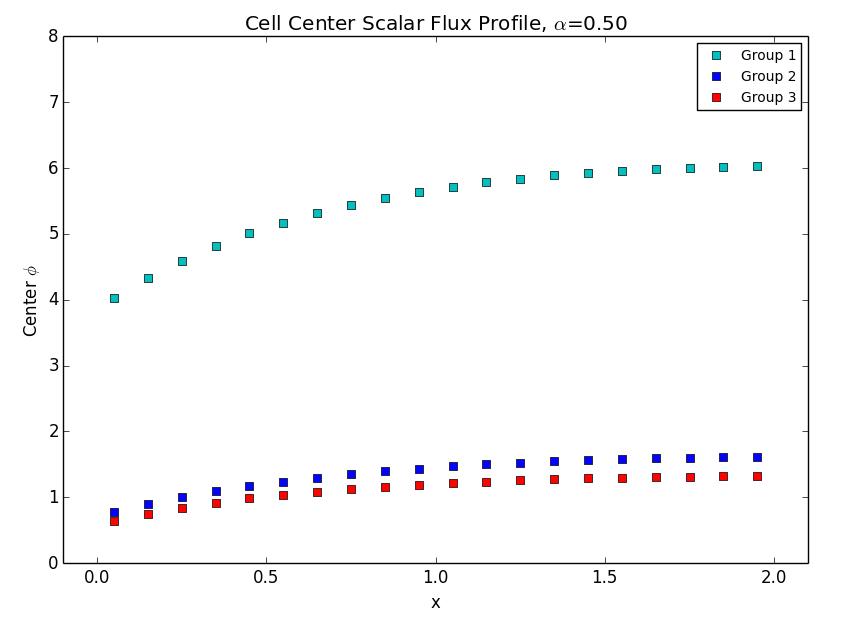
\includegraphics[width=0.6\textwidth]{Figures/groupcenterfluxes.png}
\vspace{-7pt}
\caption{Cell centered scalar flux values for groups 1, 2, and 3.}
\end{figure}

\textbf{Aside}: If we reduce the total cross-sections in group 2 and 3 (to 0.5 in each group), we see that the group 3 flux surpasses the group 2 flux (Fig.~2). This agrees with intuition, as now particles in group 2 will have a higher likelihood to scatter into group 3 and once in group 3, have a smaller likelihood to get absorbed. We also see an increase in amplitude for both group 2 and group 3, because the absorption cross-section is now lower. And again, since groups 2 and 3 have no influence on group 1, the group 1 flux is unchanged.

\begin{figure}[htb!]
\centering
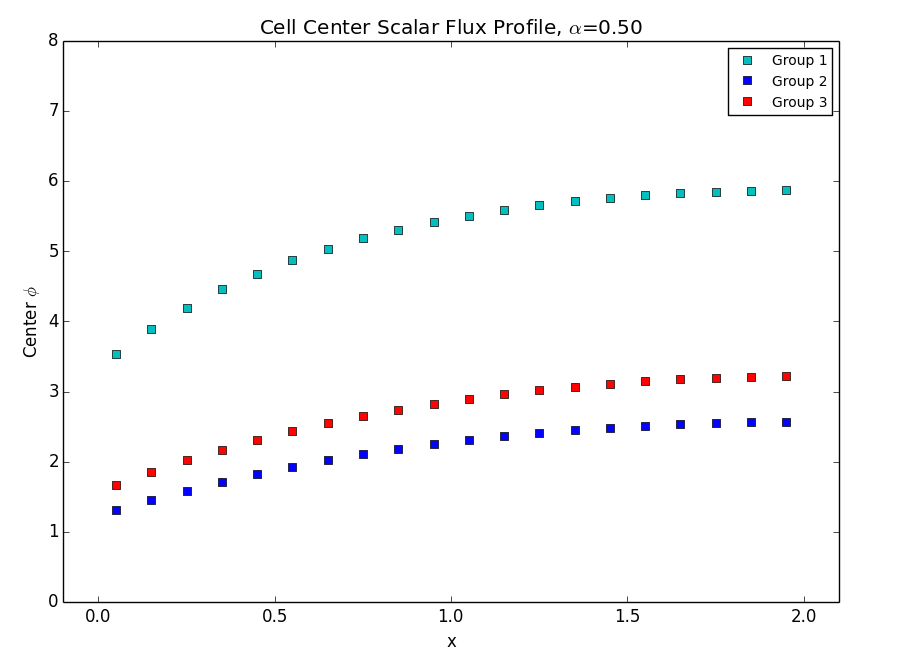
\includegraphics[width=0.6\textwidth]{Figures/groupcenterfluxes_lowertotxsection.png}
\vspace{-7pt}
\caption{Cell centered scalar flux values for groups 1, 2, and 3 using $\Sigma_t = 0.5$ in all groups.}
\end{figure}



% - - - - - - - - - - - - - - - - - - - - - - - - - - - - - - - - - - - - - - - - - -

\end{document}
